\documentclass[11pt,a4paper,austrian,titlepage,
chapterprefix,headsepline,parskip,pdftex,
,numbers=noenddot,bibliography=totoc]{scrreprt}

%%% old: \documentclass[11pt,a4paper,austrian,titlepage,
%chapterprefix,headsepline,parskip,pdftex,
%,pointlessnumbers,bibtotoc]{scrreprt}

%%% Abs‰tze bei tieferen Ebenen einschalten
\makeatletter %% Sonderbedeutung von @ aufheben
\renewcommand{\paragraph}{\@startsection
   {paragraph} % name
   {4} % ebene
   {0mm} % einzug
   {-\baselineskip} % vorabstand
   {0.1\baselineskip} % nachabstand
   {\normalfont\normalsize\bfseries}} % stil
\makeatother %% Sonderbedeutung von @ wieder

\makeatletter %% Sonderbedeutung von @ aufheben
\renewcommand{\subparagraph}{\@startsection
   {subparagraph} % name
   {5} % ebene
   {0mm} % einzug
   {-\baselineskip} % vorabstand
   {0.1\baselineskip} % nachabstand
   {\normalfont\normalsize\bfseries}} % stil
\makeatother %% Sonderbedeutung von @ wieder

\usepackage{setspace}
\onehalfspacing

\usepackage[pdftex]{graphicx}

% for colours
\usepackage[pdftex]{color}

\usepackage[colorlinks=true,
    linkcolor=black,
    citecolor=black,
%    pagecolor=black,
    urlcolor=black,
    breaklinks=true,
    bookmarksnumbered=true,
    hypertexnames=false,
    pdfpagemode=UseOutlines,
    pdfview=FitH,
    plainpages=false,
    pdfpagelabels,
    bookmarks=true,
    linktocpage=true]{hyperref}

\hypersetup{pdfauthor={Vorname Nachname},
    pdftitle={Testtitel},
    pdfsubject={Diplomarbeit},
    pdfkeywords={},
    pdfcreator={pdfLaTeX with hyperref (\today})}

%%% f¸r Source-Code
\usepackage{listings}
\lstset{language=Java}


% Interner-Link-Befehl
\newcommand{\internerLink}[1]{\hyperref[#1]
{Siehe \ref*{#1}~\nameref{#1} auf S.~\pageref{#1}}}

% Interner-Link-Befehl 2
\newcommand{\ffinternerLink}[1]{\hyperref[#1]
{Siehe S.~\pageref{#1}ff}}

% Interner-Link-Befehl x
\newcommand{\xinternerLink}[1]{\hyperref[#1]
{\ref*{#1}~\nameref{#1} auf S.~\pageref{#1}}}


%%% continous footnote
\newcounter{cfootnotecounter}
\newcommand{\cfootnote}[1]{\stepcounter{cfootnotecounter}
\footnote[\value{cfootnotecounter}]{#1}}

\flushbottom

\usepackage{geometry}
\geometry{a4paper,left=20mm, right=20mm, top=20mm, bottom=20mm, includeheadfoot}
% change page settings
	%\setlength{\hoffset}{0mm} \setlength{\voffset}{0mm}
	%\setlength{\evensidemargin}{14.6mm}
	%\setlength{\oddsidemargin}{14.6mm} \setlength{\topmargin}{-20mm}
	%\setlength{\headheight}{15mm} \setlength{\headsep}{9mm}
	%\setlength{\textheight}{242mm} \setlength{\textwidth}{145mm}
	%\setlength{\footskip}{10mm}
%%% Nachfolgendes nicht notwendig wg. Klassenoption parskip
%\setlength{\parskip}{3ex plus0.5ex minus0.5ex}
%\setlength{\parindent}{0mm}

%%% Abst‰nde von float-Umgebungen
%\setlength{\textfloatsep}{25pt plus5pt minus5pt}
%\setlength{\intextsep}{25pt plus5pt minus5pt}

%%% Gliederungs-Nummern in den Rand schreiben
%\renewcommand*{\othersectionlevelsformat}[1]{%
%\llap{\csname the#1\endcsname\autodot\enskip}}

%%% In Kopfzeile nur Kapitel-Text ohne "Kapitel x"
\renewcommand*{\chaptermarkformat}{}

%%% Formatierung von chapter ‰ndern
\setkomafont{chapter}{\Huge}
\renewcommand*{\chapterformat}
{\LARGE{\chapappifchapterprefix{\ }
\thechapter\autodot\enskip}}

%%% Kopfzeile
\usepackage[automark]{scrpage2}

\clearscrheadings \clearscrplain \clearscrheadfoot
\pagestyle{scrheadings}
\ohead{\pagemark}
\ihead{\headmark}
\cfoot{}

%%% Formatierung von Kapitel-Seiten
\renewcommand*{\chapterpagestyle}{scrheadings}

%% Gliederung TOC und Nummerierungstiefe
\setcounter{tocdepth}{\subsubsectionlevel}
\setcounter{secnumdepth}{\paragraphlevel}

%%% Array f¸r Tabellen
\usepackage{array}

%%% Schriftarten
\addtokomafont{chapter}{\sffamily}
\addtokomafont{sectioning}{\rmfamily}

% Sprache
 %\usepackage[naustrian ,ngerman]{babel} 
 \usepackage[english]{babel} 
% Eingabe von Umlauten
\usepackage[applemac]{inputenc}
% Verwenden von T1 Fonts
\usepackage[T1]{fontenc}
% \usepackage{ae}
\usepackage{lmodern}

% URLs
\usepackage{url}

%%% Einbinden von kompletten PDF-Seiten
\usepackage{pdfpages}

\usepackage{algorithmic}
\usepackage{algorithm}

\usepackage{scrhack} 

\definecolor{dkgreen}{rgb}{0,0.6,0}
\definecolor{gray}{rgb}{0.5,0.5,0.5}
\definecolor{mauve}{rgb}{0.58,0,0.82}
\usepackage{tikz}
\usetikzlibrary{shapes, arrows, positioning}
\usetikzlibrary{fit}
\usepackage{xspace}
\usepackage{todonotes}
\usepackage{color}
\usepackage{amsmath}
\usepackage{paralist}
\usepackage{tabulary}
\usepackage{subfigure}
\usepackage[all, defaultlines=3]{nowidow}
 \usepackage{cite}
\usepackage[sort]{natbib}

 
\lstset{ %
  language=java,                % the language of the code
  basicstyle=\footnotesize,           % the size of the fonts that are used for the code
  numbers=left,                   % where to put the line-numbers
  numberstyle=\tiny\color{gray},  % the style that is used for the line-numbers
  stepnumber=1,                   % the step between two line-numbers. If it's 1, each line 
                                  % will be numbered
  numbersep=5pt,                  % how far the line-numbers are from the code
  backgroundcolor=\color{white},      % choose the background color. You must add \usepackage{color}
  showspaces=false,               % show spaces adding particular underscores
  showstringspaces=false,         % underline spaces within strings
  showtabs=false,                 % show tabs within strings adding particular underscores
  frame=none,                   % adds a frame around the code
  rulecolor=\color{black},        % if not set, the frame-color may be changed on line-breaks within not-black text (e.g. commens (green here))
  tabsize=2,                      % sets default tabsize to 2 spaces
  captionpos=b,                   % sets the caption-position to bottom
  breaklines=true,                % sets automatic line breaking
  breakatwhitespace=false,        % sets if automatic breaks should only happen at whitespace
  title=\lstname,                   % show the filename of files included with \lstinputlisting;
                                  % also try caption instead of title
  keywordstyle=\color{blue},          % keyword style
  commentstyle=\color{dkgreen},       % comment style
  stringstyle=\color{mauve},         % string literal style
  escapeinside={\%*}{*)},            % if you want to add a comment within your code
  morekeywords={*,...,public,class,native}               % if you want to add more keywords to the set
}
\usepackage{courier}
\usepackage{eqparbox,array}
\renewcommand\algorithmiccomment[1]{%
 \#\ \eqparbox{COMMENT}{#1}%
}

\newcommand{\mynote}[3]{
\definecolor{tempcolor}{RGB}{#2}
{\color{tempcolor}\fbox{\bfseries\sffamily\scriptsize#1}\small\textsf\emph#3}
}

\newcommand\TODO[1]{\mynote{TODO}{0,0,255}{#1}}
\newcommand\cw[1]{\mynote{Christopher C}{255,0,0}{#1}}

\author{Christopher Warmbold}
\title{Node.js benchmark suite}


\begin{document}


%%% Titel
\pagenumbering{roman}

\includepdf{Deckblatt/coversheet.pdf}

%%% Struktur-Elemente
\pagenumbering{Roman}

\chapter*{Abstract}
This thesis presents a way to benchmark typical \textit{Node.js} applications. Node.js is a \textit{JavaScript} based runtime environment mostly for server-sided web applications. There are already existing JavaScript benchmark suites which just test the performance of the core runtime. This thesis shows how to test the performance of a typical Node.js application with its typical characteristics, such as request handling, I/O performance and VM-level performance. 

Firstly, it evaluates which packages are currently the most popular ones by analyzing the registry of the package manager \textit{npm}.
Then some of these popular packages which are considered as relevant for performance testing are used in some benchmark applications. The thesis also describes how these applications are benchmarked with \textit{Apache JMeter}.



\newpage

\chapter*{Kurzfassung}
Diese Bachelorarbeit pr\"asentiert eine M\"oglichkeit, typische \textit{Node.js} Applikationen zu benchmarken. Node.js ist eine auf \textit{JavaScript} basierende Plattform die haupts\"achlich f\"ur serverseitige Webapplikationen verwendet wird. Es gibt bereits einige JavaScript Benchmark Suiten, welche aber nur das Kern-Laufzeitverhalten testen. Diese Arbeit zeigt wie man die Performance einer typischen Node.js Applikation und ihrer typischen Charakteristiken, wie zum Beispiel das Request-Handling, die I/O Performance und die VM-Level Performance, testen kann.

Zuerst werden die derzeit popul\"arsten Pakete evaluiert, indem das Verzeichnis des Paket-Managers \textit{npm} analysiert wird. Dann werden einige dieser Pakete, welche f\"ur das durchf\"uhren eines Benchmarks relevant sind, in verschiedenen Test-Applikationen verwendet. Weiters zeigt diese Bachelorarbeit, wie man diese Applikationen mit \textit{Apache JMeter} testen und auswerten kann.


\newpage

\tableofcontents



%%% Eigentlicher Inhalt
\newpage
\pagenumbering{arabic}

\chapter{Introduction}

Node.js is a JavaScript based runtime environment mostly for server-sided web applications. To test the performance of engines executing Node.js applications some Node.js specific benchmarks are needed.

There are already some Node.js or JavaScript benchmarks but none of them test the typical characteristics of Node.js applications, such as parallel request handling, IO performance and VM-level performance.
For this reason some sample applications which behave like typical real world Node.js applications will be developed. These applications should have many dependencies to popular libraries. Therefore the package manager npm will be analyzed in order to find the most popular packages. Some of these packages which are considered as relevant for performance testing will be used within the sample applications.

The performance of the sample applications will then be tested with the help of an existing workload generator called Apache JMeter. The results of these tests will be discussed and the bottlenecks will be identified.


\chapter{Node.js Ecosystem}
\begin{quote}
\textit{Node.js}\textsuperscript{\textregistered} is a JavaScript runtime built on Chrome's V8 JavaScript engine. Node.js uses an event-driven, non-blocking I/O model that makes it lightweight and efficient. Node.js' package ecosystem, npm, is the largest ecosystem of open source libraries in the world.\cite{nodejs}
\end{quote}
\section{Packages}
Node.js has a built in package manager called \textit{nmp} (node package manager). In order to keep the Node.js core as lightweight as possible a lot of functionality comes with packages. Npm provides a public package registry where everyone can publish packages which can be used in any Node.js application\cite{npm-about}.

\subsection{Popular Packages}
\label{subsec:popular-packages}
The goal of the benchmark suite it to test the performance of the underlying Node.js runtime. This means that the benchmarks should cover typical use cases of Node.js applications. This could be archived by using the most popular npm packages within the benchmarked applications.

There are different ways of measuring the popularity of npm modules. Each npm module can get a \textit{star} from any developer. This are currently the most starred packages\cite{npm-starred}:

	\begin{longtable}{ll}
		\caption{Most starred npm packages}\\
		package&stars\\
		\hline
		\endfirsthead
		\caption[]{Most starred npm packages}\\
		package&stars\\
		\hline
		\endhead
		\textbf{express} & 1719 \\
		gulp & 1086 \\
		request & 948 \\
		async & 922 \\
		\textbf{lodash} & 857 \\
		browserify & 729 \\
		pm2 & 703 \\
		grunt & 616 \\
		\textbf{commander} & 607 \\
		socket.io & 594 \\
		forever & 541 \\
		\textbf{moment} & 532 \\
		mongoose & 514 \\
		mocha & 497 \\
		bower & 483 \\
		\textbf{chalk} & 466 \\
		underscore & 431 \\
		gulp-uglify & 416 \\
		\textbf{cheerio} & 404 \\
		debug & 398 \\
		q & 367 \\
		npm & 366 \\
		\textbf{passport} & 357 \\
		react & 356 \\
		\textbf{bluebird} & 352 \\
		gulp-concat & 352 \\
		\textbf{nodemailer} & 351 \\
		\textbf{colors} & 343 \\
		redis & 332 \\
		gulp-sass & 330 \\
	\end{longtable}
Note: All bold packages are used by the benchmarked applications (see Chapter~\ref{ch:benchmark-applications}).



Another method of measuring the popularity of packages is to find the most depended-upon packages. This are the currently the most depended-upon packages\cite{npm-depended}:

	\begin{longtable}{ll}
		\caption{Most depended-upon packages}\\
		package&stars\\
		\hline
		\endfirsthead
		\caption[]{Most depended-upon packages}\\
		package&stars\\
		\hline
		\endhead
		\textbf{lodash} & 27018 \\
		request & 16534 \\
		async & 15407 \\
		underscore & 12799 \\
		\textbf{express} & 10953 \\
		\textbf{commander} & 10816 \\
		\textbf{chalk} & 10640 \\
		debug & 9700 \\
		\textbf{bluebird} & 8754 \\
		\textbf{mkdirp} & 7147 \\
		\textbf{colors} & 6683 \\
		\textbf{moment} & 6335 \\
		through2 & 6200 \\
		q & 6129 \\
		yeoman-generator & 5497 \\
		react & 5343 \\
		\textbf{glob} & 5172 \\
		minimist & 4945 \\
		gulp-util & 4885 \\
		coffee-script & 4646 \\
		\textbf{fs-extra} & 4148 \\
		\textbf{body-parser} & 4075 \\
		jquery & 4017 \\
		\textbf{cheerio} & 3792 \\
		optimist & 3413 \\
		yargs & 3305 \\
		\textbf{node-uuid} & 2968 \\
		yosay & 2922 \\
		babel-runtime & 2919 \\
		gulp & 2915 \\
	\end{longtable}
Note: All bold packages are used by the benchmarked applications (see Chapter~\ref{ch:benchmark-applications}).

\chapter{Benchmark Applications}
\label{ch:benchmark-applications}
This chapter introduces the applications which are used by the benchmark suite. The benchmarks should test typical Node.js characteristics. Therefore these applications are using many of the popular packages from npm which were discussed Section~\ref{subsec:popular-packages}.

With Node.js it is not only possible to write web applications but also to write console applications. The benchmark suite should not test the same functionality again and again and for this reason three different applications were created:
\begin{itemize}
	\item I/O intensive application $\rightarrow$ should produce many I/O-operations
	\item CPU intensive application $\rightarrow$ should be computation heavy
	\item Rich web application $\rightarrow$ should have many dependencies and should behave like a modern web application
\end{itemize}

\section{I/O-Application}
	This console application copies all files from a given source directory to a given target directory. 
	\subsection{Usage}
	Output of \texttt{node app -{}-help}:
	\par
	\begingroup
	\leftskip=1cm
	\noindent   Usage: app sourceDir targetDir [options]
	
	  I/O-Application: copies all files from the source directory to the target directory.
	
	  Options:
	
	    -h, -{}-help                    output usage information\newline
	    -V, -{}-version                 output the version number\newline
	    -c -{}-copyfunction <function>  select copyfunction to use. fse (=fs-extra) or ncp. fallback is fse.
	\par
	\endgroup
	
	I found two popular packages, \texttt{fs-extra}\citep{fs-extra} and \texttt{ncp}\citep{ncp}, which can copy the contents of a directory recursively. I tried both of them and sometimes they were  quite different in aspect of the runtime. Because of that I decided to add the option to switch between those packages with the \texttt{-c} option. 
	
	\subsection{Used Packages}
	This application uses following packages:
	\begin{longtable}{ll}
		\caption{I/O-application dependencies}\\
		package&version\\
		\hline
		\endfirsthead
		\caption[]{I/O-application dependencies}\\
		package&version\\
		\hline
		\endhead
		colors\cite{colors} & 1.1.2 \\
		commander\cite{commander} & 2.9.0 \\
		fs-extra\cite{fs-extra} & 0.30.0 \\
		mkdirp\cite{mkdirp} & 0.5.1 \\
		ncp\cite{ncp} & 2.0.0 \\
		verror\cite{verror} & 1.6.1 \\
	\end{longtable}
	\subsection{Known Issues}
	When using this application with a huge amount of files the applications gets not only I/O intensive but also the CPU load reaches a high level.
\section{CPU-Application}
	This console application compresses and encrypts a given file or directory. It is also able to decrypt and decompress a given file. Furthermore you can choose the encryption algorithm and set the encryption password. In order to increase the CPU load it is also possible to set a count how often the encryption or decryption algorithm should be applied.
	\subsection{Usage}
	\label{subsec:cpu-usage}
	Output of \texttt{node app -{}-help}:
	\par
	\begingroup
	\leftskip=1cm
	\noindent
	Usage: app [options] <source>
	
	  CPU-Application: compress and encrypt a file/directory.
	
	  Options:
	
	    -h, -{}-help                        output usage information\newline
	    -V, -{}-version                     output the version number\newline
	    -a -{}-algorithm <cipheralgorithm>  set cipher algorithm. default: CAST-cbc\newline
	    -c -{}-count <count>                how often the cipher algorithm should be applied\newline
	    -p -{}-password <password>          set encryption password. default password is "password"
	    -d -{}-decrypt                      decrypt file
	\par
	\endgroup
	\subsection{Used Packages}
	This application uses following packages:
	\begin{longtable}{ll}
		\caption{CPU-application dependencies}\\
		package&version\\
		\hline
		\endfirsthead
		\caption[]{CPU-application dependencies}\\
		package&version\\
		\hline
		\endhead
		colors\cite{colors} & 1.1.2 \\
		commander\cite{commander} & 2.9.0 \\
		crypto\cite{crypto} & 0.0.3 \\
		fstream\cite{fstream} & 1.0.10 \\
		path\cite{path} & 0.12.7 \\
		tar\cite{tar} & 2.2.1 \\
		verror\cite{verror} & 1.6.1 \\
	\end{longtable}
	\subsection{Known Issues}
	\label{subsec:cpu-known-issues}
	Because Node.js is running single threaded the CPU load of just one core is going to rise. Node.js could support multiple cores with its \textbf{child\_process.fork() API} or with the \textbf{cluster} module but this is not implemented in this application (see Chapter~\ref{ch:future-work})\cite{nodejs-about}\cite{nodejs-childprocess}\cite{nodejs-cluster}.
	\section{Web Application}
	The goal of this application is to be as realistic as possible. This means that it should use technologies and frameworks which are used in many real world applications. Furthermore it should have many dependencies to popular third party libraries and follow the programming guidelines of Node.js. The effort to write such an application would exceed the scope of this thesis and therefore the best way to go is to use an existing platform. The currently most starred package in npm is \textit{express} (see Section~\ref{subsec:popular-packages} which is a framework for building web applications\cite{npm-starred}. For this reason this application uses a publishing platform which is based on express called \textit{ghost}\cite{ghost}\cite{ghost-git}.
	\subsection{Usage}
	To start ghost following command has to be executed inside the folder of the application: \texttt{npm start}.
	The default port is \textit{2368} and the back-end is accessible via \url{http://localhost:2368/ghost}. The application has following settings:
	
	\begin{tabular}{ll}
		Username: & benchmark.suite@jku.at\\
		Password: & password\\
		Public API: & enabled  \\
	\end{tabular}
	
	\subsection{Used Packages}
	This application only uses ghost\cite{ghost-npm}. But ghost itself has many dependencies:

	\begin{longtable}{ll}
		\caption{Ghost dependencies}\\
		package&version\\
		\hline
		\endfirsthead
		\caption[]{Ghost dependencies}\\
		package&version\\
		\hline
		\endhead
		amperize & 0.3.1 \\
		archiver & 1.1.0 \\
		bcryptjs & 2.3.0  \\
		bluebird & 3.4.6 \\
		body-parser & 1.15.2 \\
		bookshelf & 0.10.1 \\
		chalk & 1.1.3 \\
		cheerio & 0.22.0 \\
		compression & 1.6.2 \\
		connect-slashes & 1.3.1 \\
		cookie-session & 1.2.0 \\
		cors & 2.8.1 \\
		csv-parser & 1.11.0 \\
		downsize & 0.0.8 \\
		express & 4.14.0 \\
		express-hbs & 1.0.3 \\
		extract-zip-fork & 1.5.1 \\
		fs-extra & 0.30.0 \\
		ghost-gql & 0.0.5 \\
		glob & 5.0.15 \\
		gscan & 0.0.15 \\
		html-to-text & 2.1.3 \\
		image-size & 0.5.0 \\
		intl & 1.2.5 \\
		intl-messageformat & 1.3.0 \\
		jsonpath & 0.2.7 \\
		knex & 0.12.2 \\
		lodash & 4.16.0 \\
		moment & 2.15.1 \\
		moment-timezone & 0.5.5 \\
		morgan & 1.7.0 \\
		multer & 1.2.0 \\
		netjet & 1.1.3 \\
		node-uuid & 1.4.7 \\
		nodemailer & 0.7.1 \\
		oauth2orize & 1.5.0 \\
		passport & 0.3.2 \\
		passport-http-bearer & 1.0.1 \\
		passport-oauth2-client-password & 0.1.2 \\
		path-match & 1.2.4 \\
		rss & 1.2.1 \\
		sanitize-html & 1.13.0 \\
		semver & 5.3.0 \\
		showdown-ghost & 0.3.6 \\
		sqlite3 & 3.1.4 \\
		superagent & 2.3.0 \\
		unidecode & 0.1.8 \\
		validator & 5.7.0 \\
		xml & 1.0.1 \\
	\end{longtable} 	
	
	\subsection{Known Issues}
	As mentioned in Section~\ref{subsec:cpu-known-issues}, Node.js is not supporting multiple cores by default. Because of that ghost can not handle parallel requests. This causes requests to wait till the previous requests are finished. It is possible to scale ghost with the cluster module but this is not implemented in the benchmark suite (see Chapter~\ref{ch:future-work})\cite{ghost-cluster}\cite{nodejs-cluster}.
	
	
	First I tried to add ghost as npm module\cite{ghost-module}. In order to start ghost you have to install all dependencies by calling \texttt{npm install}. This command will download ghost and  all its dependencies inside the \textit{node\_modules} folder. The \textit{content} folder where the configuration and the database are saved are then also located inside the \textit{node\_modules} folder. Typically you add \textit{node\_modules} to your \textit{.gitignore} file so that these files are not uploaded to the git repository but in this case where you want to keep the stored configuration and database you have to include it. Ghost has many dependencies and this causes very long filenames inside this folder unfortunately the windows git client has a small character limit for filenames as a result you might not be able to push or pull from the git repository. This limit could be bypassed by editing the git configuration with the \texttt{git config -{}-system core.longpaths true} command but I decided to switch to the standalone ghost release where the \textit{content} folder is not placed inside the \textit{node\_modules} folder and so this folder can be excluded from git.
\chapter{Benchmark System}
The goal of the benchmark system is to test the applications described in Chapter~\ref{ch:benchmark-applications} under realistic workload conditions. For this reason the benchmark system uses an existing workload generation tool called \textit{Apache JMeter}\cite{jmeter}. Furthermore an utility script which wraps all together and starts the benchmarks is provided.
\section{Apache JMeter}
\label{sec:apache-jmeter}
Apache JMeter is an open source load testing tool written in Java. It is a powerful tool to generate workload and measure the performance of any static or dynamic resource (Webservices, Web dynamic languages - PHP, Java, ASP.NET, Files, Java Objects, Data Bases and Queries, FTP Servers and more)\cite{jmeter}.

JMeter can send predefined HTTP requests to the Node.js applications and measure the response time. It is possible to set how often these requests should be looped or how many threads should send the predefined requests simultaneously to simulate multiple parallel user requests.
\section{Web Application Wrapper}
As mentioned in Section~\ref{sec:apache-jmeter} the applications need to be accessible via HTTP but as described in Chapter~\ref{ch:benchmark-applications} the benchmark suite contains two console applications. For this reason a web application wrapper was developed. This wrapper application wraps a given console application and starts a web server where the console application can be accessed. The console parameters can be passed in the query string of a request. The console application is called synchronously in order to measure the execution time and the results are sent to the HTTP client. This allows the benchmarking suite only to measure the response time of the requests. 

\subsection{Usage}
	Output of \texttt{node app -{}-help}:
	\par
	\begingroup
	\leftskip=1cm
	\noindent
	Usage: app [options] <source>
	
	  Webserver-Wrapper-Application: wraps a console application in a web application.
	
	  Options:
	
	    -h, -{}-help                      output usage information\newline
	    -V, -{}-version                   output the version number\newline
	    -a -{}-application <application>  set the application which should be wrapped\newline
	    -p -{}-port <port>                set the port of the web server
	\par
	\endgroup
	
	Example: 
	
	
	The following example starts the I/O application on port 8081. \\
	\texttt{node webserver-wrapper\textbackslash app.js -a "node io-application\textbackslash app.js" -p 8081} \\
	
	
	Sample Requests:

	The following examples show how to pass parameters to the application.\\
	\texttt{\url{http://localhost:8081?args=--help}} \\
	\texttt{\url{http://localhost:8081?args=sourceDir\%20targetDir}} \\ 
	
\subsection{Used Packages}
This application uses following packages:
\begin{longtable}{ll}
		\caption{Web Application Wrapper dependencies}\\
		package&version\\
		\hline
		\endfirsthead
		\caption[]{Web Application Wrapper dependencies}\\
		package&version\\
		\hline
		\endhead
		child\_process & 1.0.2 \\
		colors & 1.1.2 \\
		commander & 2.9.0 \\
		express & 4.14.0 \\
\end{longtable}

\section{Sample Files}
Two of the applications described in Chapter~\ref{ch:benchmark-applications} need files or a folder as input. Therefore the benchmark suite contains some sample files such as audio files, video files, documents and an empty ghost application. The files should represent real data. The empty ghost application was added because it has a big file structure with more than 400 files (without dependencies). 

Source of the media files: \url{https://kodi.tv/media-samples/}

This sample-data folder ensures that the tests have the same conditions and work with the same data. The contents of this folder can be modified because the benchmarks always use the whole folder for its requests but it should stay the same when you want to compare the results.
\section{Benchmarks}
\label{sec:benchmarks}
	\subsection{I/O-Application}
	\label{subsec:io-bechmark}
	Following scenarios are covered by the benchmark:
	\begin{itemize}
		\item copy sample-data to \textit{tmp\textbackslash io\_<threadId>\_<loopCounter>}
		\item copy sample-data to \textit{tmp\textbackslash io\_<threadId>\_<loopCounter>} with ncp as copy library
	\end{itemize}
	
	To prevent different threads and loop iterations from copying to the same folder the thread-id and the loop-counter are added to the target directory folder.
	
	The test cases above are executed in different ways:
	\begin{itemize}
		\item looped 10 times in 1 thread $\rightarrow$ total 10 times
		\item executed once in 10 threads with a ramp-up period of 1 second  $\rightarrow$ total 10 times
	\end{itemize}
	The ramp-up period tells JMeter how long to take till all threads are started. For example if 30 threads are used and the ramp-up period is 10 seconds, JMeter will start all 30 threads within 10 seconds.
	\subsection{CPU-Application}
	\label{subsec:cpu-bechmark}
		Following scenarios are covered by the benchmark:
	\begin{itemize}
		\item compress sample-data to \textit{tmp\textbackslash cpu\_<threadId>\_<loopCounter>}
		\item compress sample-data to \textit{tmp\textbackslash cpu\_c5\_<threadId>\_<loopCounter>} with encryption count 5
	\end{itemize}
	
	To prevent different threads and loop iterations from writing to the same folder the thread-id and the loop-counter are added to the target directory folder.
	
	The test cases above are executed in different ways:
	\begin{itemize}
		\item looped 10 times in 1 thread $\rightarrow$ total 10 times
		\item executed once in 10 threads with a ramp-up period of 1 second  $\rightarrow$ total 10 times
	\end{itemize}
	The ramp-up period tells JMeter how long to take till all threads are started. For example if 30 threads are used and the ramp-up period is 10 seconds, JMeter will start all 30 threads within 10 seconds.
	\subsection{Web Application}
	\label{subsec:web-bechmark}
	Following scenario is covered by the benchmark:
	\begin{enumerate}
		\item go to the sign-in page
		\item get an access\_token (has to be extracted and stored in a JMeter variable in order to use it for future requests)
		\item navigating through the back-end
		\item open the creation view of a new article
		\item add some text to the new article. Ghost sends some AJAX requests during typing $\rightarrow$ these requests were recorded and are simulated during the benchmark. The id of the created post has also to be extracted and stored in a JMeter variable.
		\item publish the post
		\item navigate to the main page where new posts are displayed
	\end{enumerate}
	
	The test cases above are executed in different ways:
	\begin{itemize}
		\item looped 30 times in 1 thread $\rightarrow$ total 30 times
		\item executed once in 30 threads with a ramp-up period of 10 second  $\rightarrow$ total 30 times
	\end{itemize}
	The ramp-up period tells JMeter how long to take till all threads are started. For example if 30 threads are used and the ramp-up period is 10 seconds, JMeter will start all 30 threads within 10 seconds.	
	
	
	The database of ghost has to be cleared to ensure the same conditions for future benchmarks. Ghost offers a "Delete all Content" button in the back-end. Therefore a separate JMeter testplan was created which sends a request to this page. It is executed at the end of a benchmark.
\section{Utility Script}
\label{sec:utility-script}
The utility script wraps all benchmarks together and it also handles the startup of the sample applications described in Chapter~\ref{ch:benchmark-applications}.

Following steps are included:
\begin{enumerate}
	\item install the npm packages of all applications
	\item start the ghost application
	\item start a web server wrapper for the I/O-application on port 8081
	\item start a web server wrapper for the CPU-application on port 8082
	\item wait 15 seconds for all servers to startup
	\item execute the I/O-application benchmarks looped
	\item delete the \textit{tmp} folder
	\item execute the I/O-application benchmarks threaded
	\item delete the \textit{tmp} folder
	\item execute the CPU-application benchmarks looped
	\item delete the \textit{tmp} folder
	\item execute the CPU-application benchmarks threaded
	\item delete the \textit{tmp} folder
	\item execute the ghost benchmarks looped
	\item clear the ghost database
	\item execute the ghost benchmarks threaded
	\item clear the ghost database
\end{enumerate}

\textbf{Caution:} The JMeter binary folder has to be added to the PATH environment variable.\\ \\
All the JMeter test are started with following command:\\
\texttt{\$ jmeter -n -t <pathToTestplan> -l results\textbackslash output\_<testPlanName>.jtl}


	\subsection{Usage}
	The utility script can be executed in a terminal with: \\
	\texttt{\$ startBenchmark}
	
	The results are saved in the \textit{results} folder.
\chapter{Results}
\label{ch:results}
As described in Section~\ref{sec:utility-script}, JMeter testplans can be executed on the command line. But for this chapter the JMeter GUI is used because it allows to generate graphs and it can summarize the results of a test. Each benchmark described in Section~\ref{sec:benchmarks} can be opened with the JMeter GUI. The .jmx files are placed under \texttt{jmeter\textbackslash <application-name>}.

\section{Test Setup}
The following benchmarks were executed with the official Node.js runtime.\\ \\
Following setup was used:\\ \\
\begin{tabular}{ll}
	CPU & Intel Core i5-4690K (4 x 3.5 GHz) \\
	RAM & 8GB \\
	Storage & Samsung SSD 830 128GB \\
	GPU & Nvidia Geforce GTX 960 \\
	OS & Windows 10 Pro \\
	Node & Version 4.2.3 \\
	NPM & Version 3.10.8 \\
\end{tabular}
\section{I/O-Application}
As described in Section~\ref{subsec:io-bechmark} the benchmarks are performed multi-threaded and looped.

\subsection{Looped}
In this test the benchmarks are executed 10 times in 1 thread. \\

\begin{figure}[!h]
  \caption{Results view of I/O-application when executed synchronously}
  \centering
    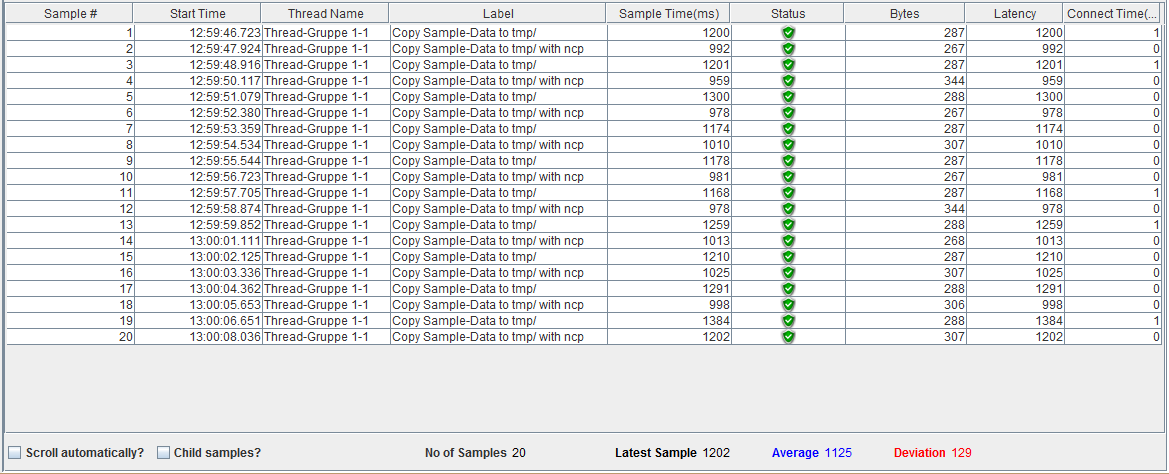
\includegraphics[width=1\textwidth]{Screenshots/io-results-looped}
    \label{fig:io-results-looped}
\end{figure}

\begin{figure}[!h]
  \caption{Aggregate Graph of I/O-application when executed synchronously}
  \centering
    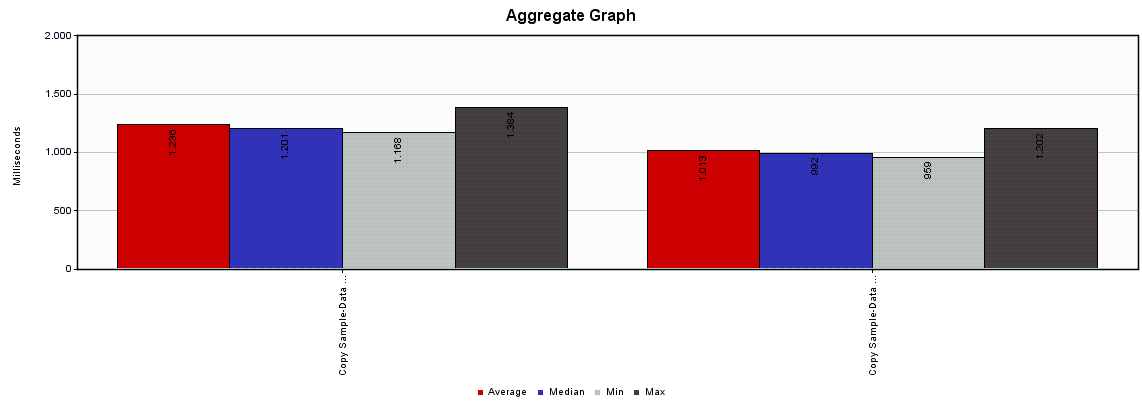
\includegraphics[width=1\textwidth]{Screenshots/io-graph-looped}
    \label{fig:io-graph-looped}
\end{figure}

In Figure~\ref{fig:io-results-looped} you see the requests JMeter has generated and in Figure~\ref{fig:io-graph-looped} you see the aggregated results. The aggregated results show that copying with the \texttt{ncp} library is slightly faster than with the \texttt{fs-extra} library.


\subsection{Multi-threaded}
\label{subsec:io-results-threaded}
In this test the benchmarks are executed once in 10 threads with a ramp-up time of 1 second. 

\begin{figure}[!h]
  \caption{Results view of I/O-application when executed parallel}
  \centering
    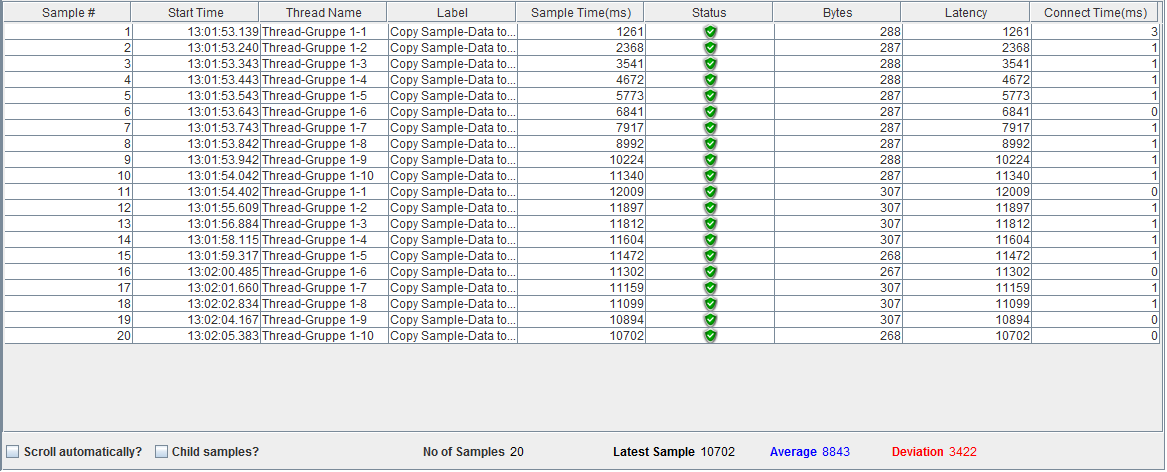
\includegraphics[width=1\textwidth]{Screenshots/io-results-threaded}
    \label{fig:io-results-threaded}
\end{figure}

\begin{figure}[!h]
  \caption{Aggregate Graph of I/O-application when executed parallel}
  \centering
    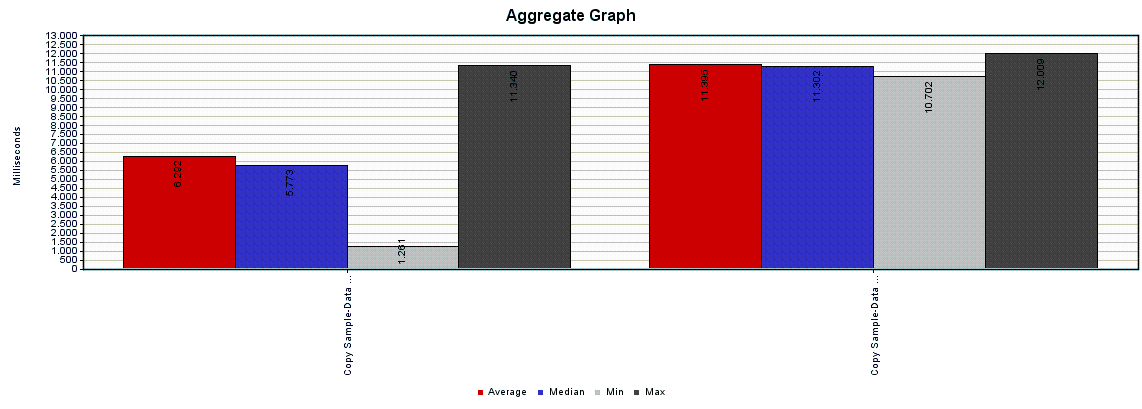
\includegraphics[width=1\textwidth]{Screenshots/io-graph-threaded}
	\label{fig:io-graph-threaded}
\end{figure}

In Figure~\ref{fig:io-results-threaded} and in Figure~\ref{fig:io-graph-threaded} you can see that Node.js is single threaded and therefore multiple requests at the same time are queued and handled synchronously. Each request has to wait for the previous requests to finish, this increases the response time. Furthermore you can see that JMeter sent the request where \texttt{ncp} is used as copy function later than the request where \texttt{fs-extra} is used. Because of this the minimum response time of the \texttt{ncp} copy requests is above 10 seconds.

\section{CPU-Application}
As described in Section~\ref{subsec:cpu-bechmark} the benchmarks are performed multi-threaded and looped.

\subsection{Looped}
In this test the benchmarks are executed 10 times in 1 thread. 

\begin{figure}[!h]
  \caption{Results view of CPU-application when executed synchronously}
  \centering
    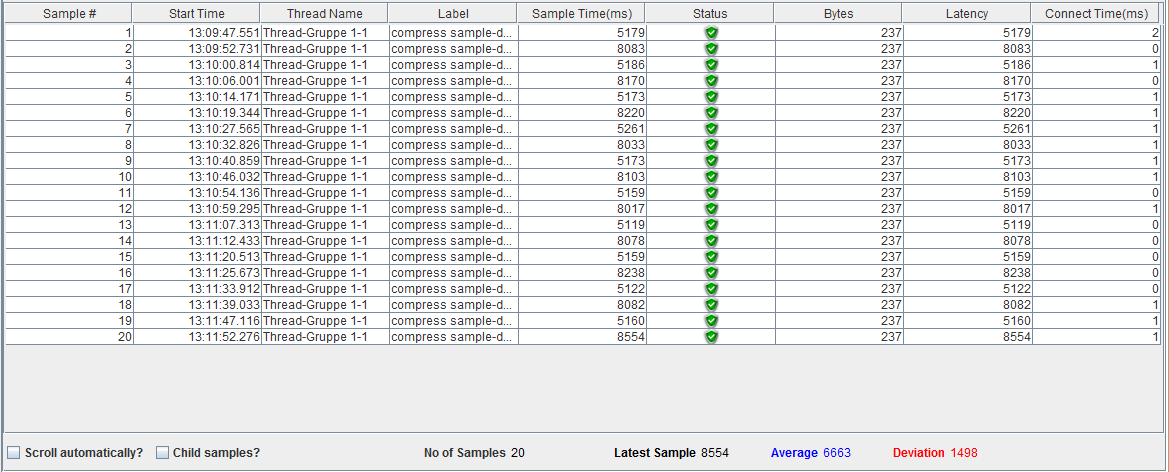
\includegraphics[width=1\textwidth]{Screenshots/cpu-results-looped}
    \label{fig:cpu-results-looped}
\end{figure}

\begin{figure}[!h]
  \caption{Aggregate Graph of CPU-application when executed synchronously}
  \centering
    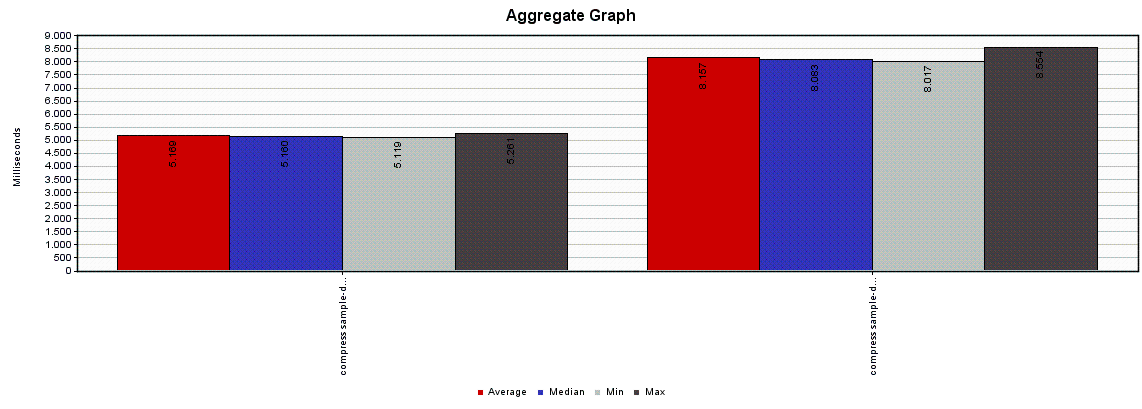
\includegraphics[width=1\textwidth]{Screenshots/cpu-graph-looped}
    \label{fig:cpu-graph-looped}
\end{figure}

In Figure~\ref{fig:cpu-results-looped} you see the requests JMeter has generated and in Figure~\ref{fig:cpu-graph-looped} you see the aggregated results. The aggregated results show that request where the encryption counter (see Section~\ref{subsec:cpu-usage}) is set to 5 have a longer response time and therefore a longer computation time than the requests where the files are only encrypted once.


\subsection{Multi-threaded}
In this test the benchmarks are executed once in 10 threads with a ramp-up time of 1 second. 

\begin{figure}[!h]
  \caption{Results view of CPU-application when executed parallel}
  \centering
    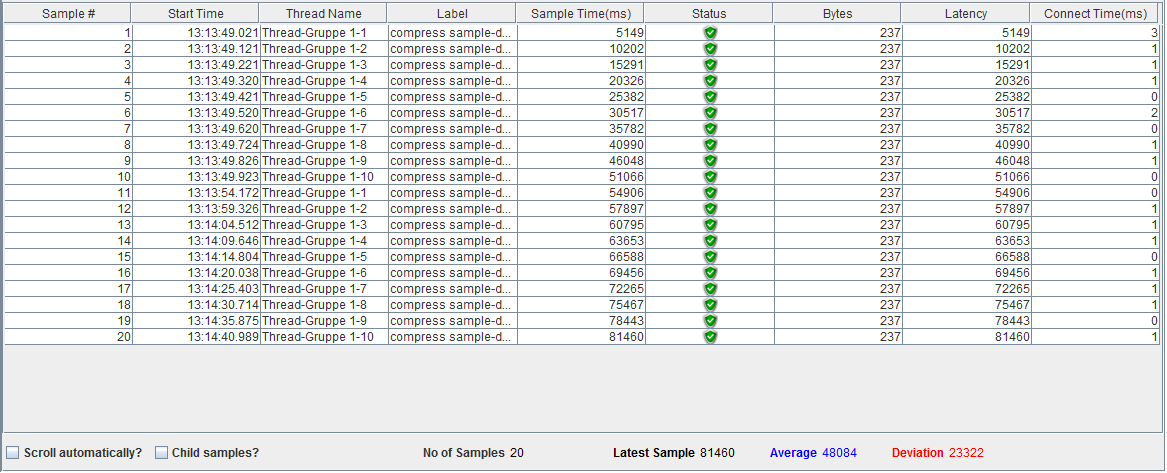
\includegraphics[width=1\textwidth]{Screenshots/cpu-results-threaded}
\end{figure}

\begin{figure}[!h]
  \caption{Aggregate Graph of CPU-application when executed parallel}
  \centering
    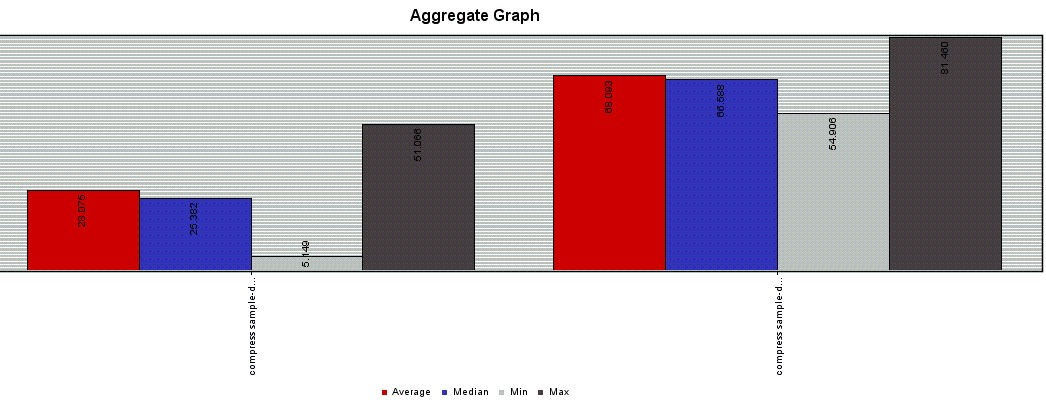
\includegraphics[width=1\textwidth]{Screenshots/cpu-graph-threaded}
\end{figure}

As described in Section~\ref{subsec:io-results-threaded} you see that the application is not optimized for multiple requests at the same time. All requests are queued and handled synchronously.

\section{Web Application}
As described in Section~\ref{subsec:web-bechmark} the benchmarks are performed multi-threaded and looped.

\subsection{Looped}
In this test the benchmarks are executed 30 times in 1 thread. 

\begin{figure}[!h]
  \caption{Results view of ghost when executed synchronously}
  \centering
    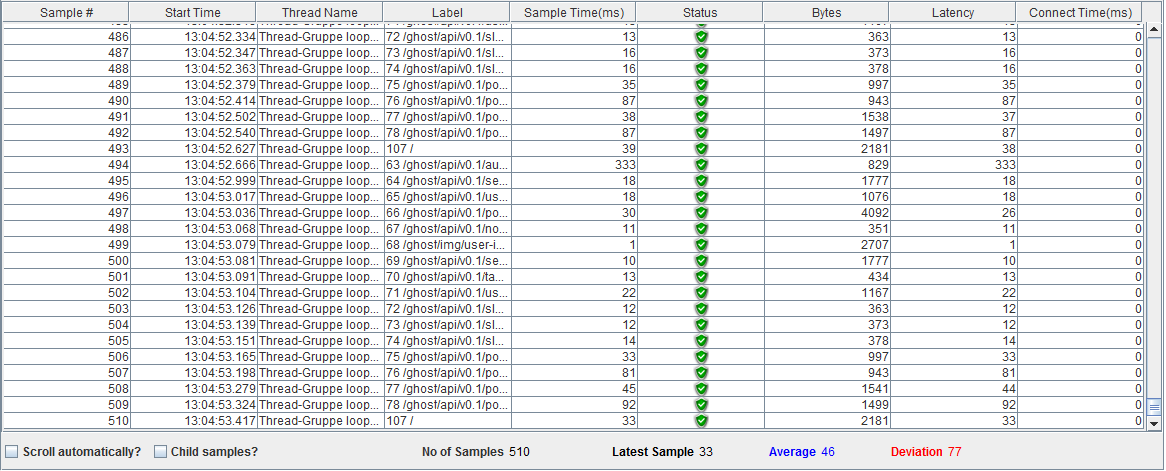
\includegraphics[width=1\textwidth]{Screenshots/web-results-looped}
    \label{fig:web-results-looped}
\end{figure}

\begin{figure}[!h]
  \caption{Report of ghost when executed synchronously}
  \centering
    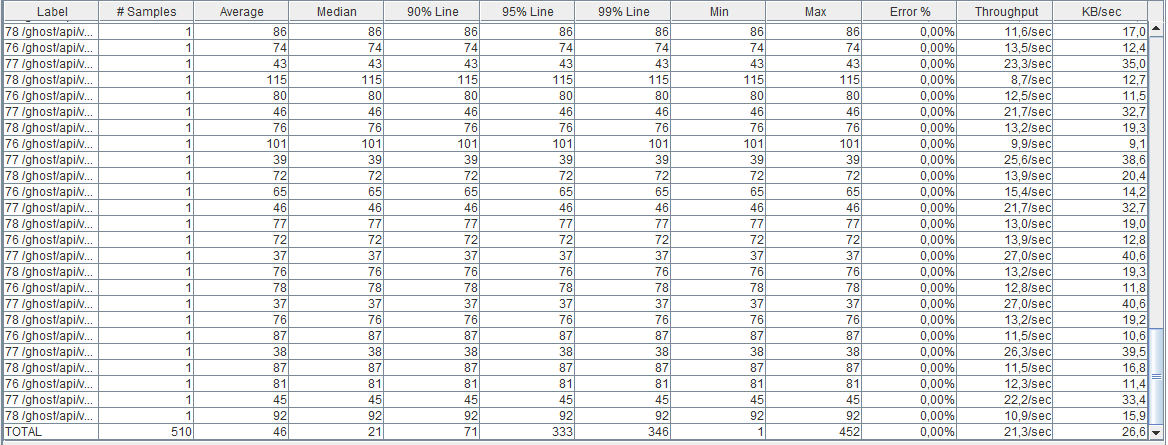
\includegraphics[width=1\textwidth]{Screenshots/web-report-looped}
	\label{fig:web-report-looped}
\end{figure}

In Figure~\ref{fig:web-results-looped} you can see the last 25 of 510 samples. In Figure~\ref{fig:web-report-looped} you see the report of the different requests. The last line of Figure~\ref{fig:web-report-looped} shows the summary of all requests. \\ \\
Following metrics might be interesting: \\
\begin{longtable}{ll}
	\caption{Ghost results looped}\\
	metric&value\\
	\hline
	\endfirsthead
	\caption[]{Ghost results looped}\\
	metric&value\\
	\hline
	\endhead
	Throughput & 21.3/sec \\
	Average & 46ms \\
	Median & 21ms \\
	Min & 1ms \\
	Max & 452ms \\
	Error & 0\% \\
\end{longtable}

\subsection{Multi-threaded}
In this test the benchmarks are executed once in 30 threads with a ramp-up time of 10 second. 

\begin{figure}[!h]
  \caption{Results view of ghost when executed parallel}
  \centering
    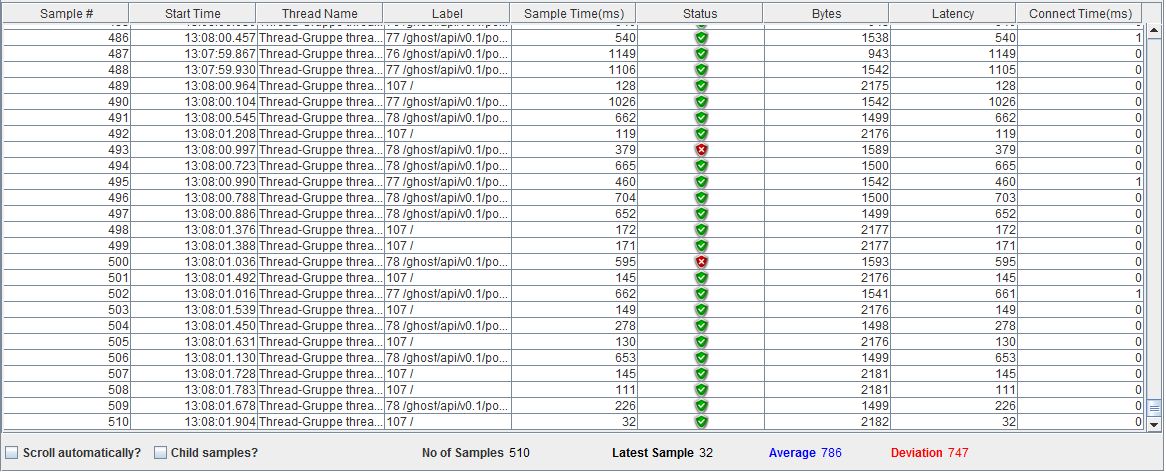
\includegraphics[width=1\textwidth]{Screenshots/web-results-threaded}
   	\label{fig:web-results-threaded}
\end{figure}

\begin{figure}[!h]
  \caption{Report of ghost when executed parallel}
  \centering
    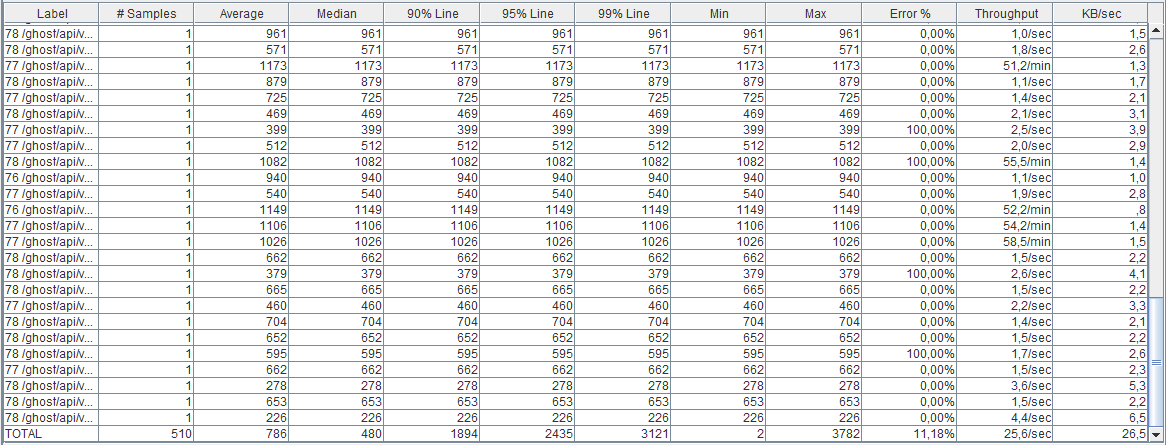
\includegraphics[width=1\textwidth]{Screenshots/web-report-threaded}
   	\label{fig:web-report-threaded}
\end{figure}

In Figure~\ref{fig:web-results-threaded} you can see the last 25 of 510 samples. In Figure~\ref{fig:web-report-threaded} you see the report of the different requests. The last line of Figure~\ref{fig:web-report-looped} shows the summary of all requests. \\ \\
Following metrics might be interesting: \\
\begin{longtable}{ll}
	\caption{Ghost results multi-threaded}\\
	\label{tab:ghost-results-multi-threaded}
	metric&value\\
	\hline
	\endfirsthead
	\caption[]{Ghost results multi-threaded}\\
	metric&value\\
	\hline
	\endhead
	Throughput & 22.6/sec \\
	Average & 786ms \\
	Median & 480ms \\
	Min & 2ms \\
	Max & 3782ms \\
	Error & 11.18\% \\
\end{longtable}

As shown in Table~\ref{tab:ghost-results-multi-threaded} ghost is not able to handle many requests at the same time and this causes some requests to fail.

\chapter{Related Work}
There are already some other Node.js benchmarks available. Following benchmarks are related to the benchmarks of this thesis:

\begin{enumerate}
	\item Acmeair (\url{https://github.com/acmeair/acmeair-nodejs}) is an existing Node.js benchmark. It tests the performance of a big Node.js application. The applications in this thesis are smaller but they cover more use cases such as I/O intensive and CPU intensive applications.
	\item Node.js Core benchmarks $\rightarrow$ these micro benchmarks cover only some core runtime performance tests, such as testing the performance of event emitters. The benchmarks in this thesis cover more than only testing some core runtime characteristics because the benchmarked applications use the most popular packages and behave like real world applications.
\end{enumerate}



\chapter{Future Work}
\label{ch:future-work}
This thesis showed how to benchmark Node.js applications but there might be some improvements possible. 

Firstly, the sample applications could be extended to support the Node.js cluster module. This module enables parallel request handling. Of course the multi-threaded benchmarks would then be faster but the benchmarks would then also cover the cluster module which is essential for many productive Node.js applications.

The results in Chapter~\ref{ch:results} cover only the official Node.js runtime. In order to compare these results the benchmarks have to be executed in different JavaScript engines with the same test setup. A possible runtime would be \textit{Graal.js} which is part of the \textit{Graal} framework\cite{graal}.



\chapter{Conclusion}

This thesis showed how to benchmark typical Node.js applications. First of all, the currently most popular packages were evaluated by analyzing the npm registry. Then some of these packages which are considered as relevant for performance testing were used in three different sample applications. These applications should represent typical use cases such as I/O intensive applications, CPU intensive applications and modern rich web applications. Then the previous developed applications were benchmarked with the help of an existing workload generator called Apache JMeter. The results were discussed in detail and the bottlenecks were identified by analyzing the results. Finally, possible future improvements were presented.



%%% Anhang
\appendix

\listoffigures
\listoftables
\bibliographystyle{plain}
\bibliography{Struktur/literature}
\chapter*{Eidesstattliche Erkl\"arung}
\markright{Eidesstattliche Erkl\"arung}

Ich erkl\"are an Eides statt, dass ich die vorliegende Bachelorarbeit selbstst\"andig und ohne fremde Hilfe verfasst, andere als die angegebenen Quellen und Hilfsmittel nicht benutzt bzw. die w\"ortlich oder sinngem\"a{\ss} entnommenen Stellen als solche kenntlich gemacht habe.

Linz, am 15. Oktober 2016

\hfill Christopher Warmbold


\end{document}
